\documentclass[12pt]{article}

\usepackage{xcolor}
\usepackage{graphicx}
\usepackage[left=1.5cm,top=2.5cm,right=1.5cm,bottom=2.5cm,bindingoffset=0.5cm]{geometry}

\usepackage{dsfont}
\usepackage{amsmath}
\usepackage[mathlines]{lineno}% Enable numbering of text and display math
\DeclareMathOperator{\Tr}{Tr}
\usepackage{url}
\usepackage[normalem]{ulem}
\usepackage{multicol, caption}
\usepackage{braket}
\bibliographystyle{elsarticle-num}

\makeatletter
\def\ps@pprintTitle{%
	\let\@oddhead\@empty
	\let\@evenhead\@empty
	\let\@oddfoot\@empty
	\let\@evenfoot\@oddfoot
}
\makeatother
\makeatletter
\makeatother

\newenvironment{Figure}
  {\par\medskip\noindent\minipage{\linewidth}}
  {\endminipage\par\medskip}

\begin{document}


\title{Matrix Product States}
%
%
% author names and IEEE memberships
% note positions of commas and nonbreaking spaces ( ~ ) LaTeX will not break
% a structure at a ~ so this keeps an author's name from being broken across
% two lines.
% use \thanks{} to gain access to the first footnote area
% a separate \thanks must be used for each paragraph as LaTeX2e's \thanks
% was not built to handle multiple paragraphs
%
\author{Glenn~LeBlanc,
Karthik~Siva
\thanks{This project was part of the Berkeley Physics Directed
Reading Program, which allows undergraduates to explore novel
material under the auspices of a graduate student mentor. K. Siva
very graciously directed this project.}}

\maketitle
\begin{multicols}{2}

\section*{Introduction}
	\subsection*{Many-Body Wavefunctions as Tensors}
		Consider a spin-$\frac{1}{2}$ particle. The particle's state is given by
		$\ket{\psi}\in\mathds{C}^2$, and for some computational basis
		$\{\ket{0}, \ket{1}\}$ we can write
		$$\ket{\psi}=\alpha\ket{0}+\beta\ket{1}$$
		with
		$$|\alpha|^2+|\beta|^2=1.$$
		This is the principle of superpostion-- the particle is superposed
		between the two basis states $\ket{0}$ and $\ket{1}$. Now if we add
		a second spin-$\frac{1}{2}$ particle, the many-body system
		$\ket{\Psi}$ is in some superposition of the four states
		$$\ket{\Psi}=\alpha\ket{00}+\beta\ket{01}+\gamma\ket{10}+\delta\ket{11}.$$
		Generally, for $N$ qubits (qudits) the system is fully
		parameterized by $2^N$ ($d^N$) complex numbers:
		$\ket{\Psi}\in\mathds{C}^{2^N}$. Notice the exponential scaling
		here. It is useful also to notice the natural bijection between
		the two spaces
		$$\mathds{C}^{2^N}\longleftrightarrow \mathds{C}^{2\times\cdots\times 2}$$
		meaning we can instead conceptualize $\ket{\Psi}$ as a
		\textit{tensor}:
		$$\ket{\Psi}\in\mathds{C}^{2\times\cdots\times2}$$
		where in this paper a tensor $\Psi$ is just a multidimensional
		array with some number of indices such that plugging in an
		assignment for each index spits out a complex number. More
		succinctly,
		$$\Psi_{i_1,i_2,\cdots,i_N}\in\mathds{C}$$
		A \textit{contraction} between two tensors $\Psi$ and $\Phi$ is
		a summation over a shared index:
		$$T_{i,j,l,m}=\sum_k\Psi_{i,j,k}\Phi_{l,k,m}$$
		is an example of a contraction. Note that dot products, matrix
		multiplication, and trace are all different vestiges of tensor
		contraction:
				\begin{align*}
				a\cdot b &=\sum_ka_kb_k\\
				(Ax)_{i} &=\sum_kA_{ik}x_k\\
				\Tr(A)&=\sum_kA_{kk}
			\end{align*}


	\subsection*{Tensor Networks}
	A \textit{tensor network} is an undirected graph whose nodes
	represent tensors and whose edges correspond to tensor indices. An
	edge between two tensors corresponds to a contraction along the
	depicted axis of each tensor. Use of this graphical language for
	representing quantum systems is attractive since it unveils relevant
	entanglement properties~\cite{TnIntro}.
	\begin{Figure}
		\center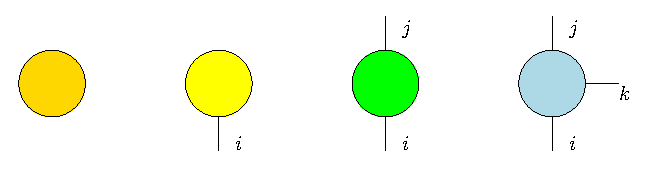
\includegraphics[width=.9\textwidth]{./Figures/tensors.eps}
		\captionof{figure}{A graphical depiction of a scalar $c$, vector
		    $v_i$, matrix $M_{ij}$, and a tensor $T_{ijk}$ of rank three.}
		\label{tensor-graphics}
	\end{Figure}
	See figure~\ref{tensor-graphics} for a graphical depiction of
	tensors of rank zero to three. Each tensor is denoted as a node with
	free edges representing each index.

	Figure~\ref{tensor-contractions} depicts the previous examples (dot
	product, matrix multiplication, trace) of tensor contraction using
	this graphical language.
	\begin{Figure}
		\center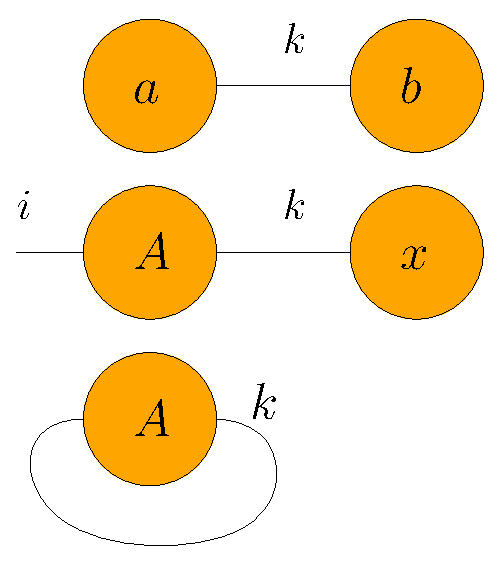
\includegraphics[width=.5\textwidth]{./Figures/contractions.eps}
		\captionof{figure}{A graphical depiction of three examples of
		    tensor contraction.}
		\label{tensor-contractions}
	\end{Figure}
	An example of an insight this graphical language provides is in
	proving trace cyclicality. The standard proof is as follows:
	\begin{align*}
		\Tr(ABC)&=\sum_{ijk}A_{ij}B_{jk}C_{ki}\\
						&=\sum_{ijk}C_{ki}A_{ij}B_{jk}\\
						&=\Tr(CAB)
	\end{align*}
	The tensor network proof is depicted in figure~\ref{trace}:
	\begin{Figure}
		\center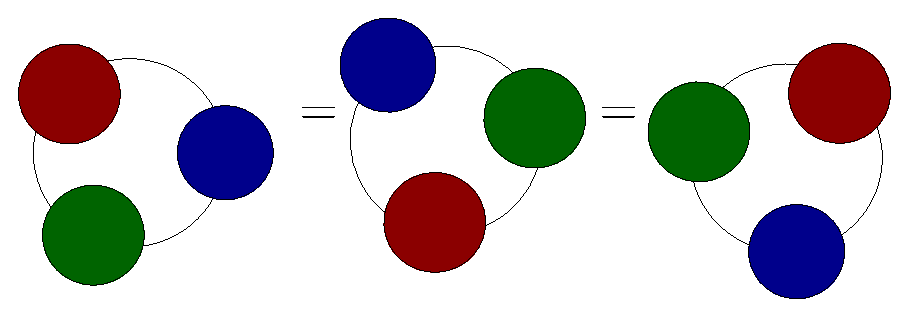
\includegraphics[width=.7\textwidth]{./Figures/trace.eps}
		\captionof{figure}{Proof of trace cyclicality.}
		\label{trace}
	\end{Figure}
	The graphical depiction of trace provides simpler insight into the
	cyclic structure of the underlying tensor contractions required to
	calculate $\Tr(ABC)$, and thus allows for a totally visual and
	immediately obvious proof of the invariance of trace under
	cyclic permutations of $A$, $B$, and $C$.



\section*{Matrix Product States}
	A \textit{matrix product state} (MPS) is a particular class
	of
	tensor network consisting of a chain of tensors each having one
	dangling edge and a bond between their nearest neighbors. See figure
	\ref{mps-example} for an example of a MPS with three sites with
	periodic and nonperiodic boundary conditions. From here we only
	consider MPS with nonperiodic boundary conditions.
	\begin{Figure}
		\center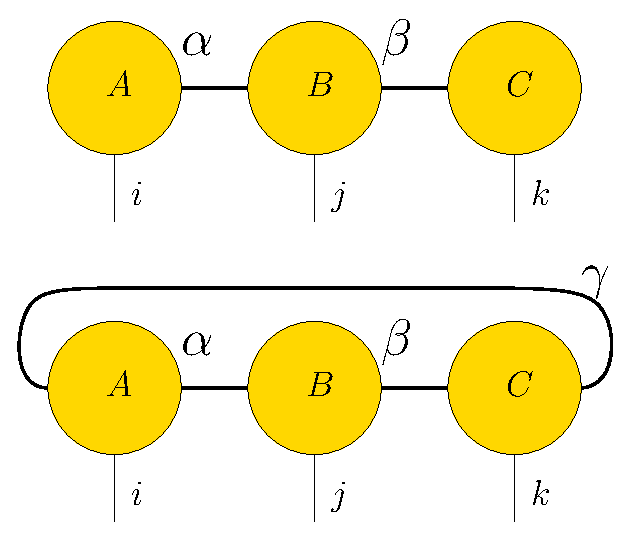
\includegraphics[width=.7\textwidth]{./Figures/mps-example.eps}
		\captionof{figure}{Two three-site MPS, the first lacking periodic boundary conditions and the second with periodic boundary conditions.}
		\label{mps-example}
	\end{Figure}
	The indices $\chi_i$ in figure~\ref{mps-example} are called
	\textit{bond indices} and are associated with a
	\textit{bond dimension}. The free indices $i,j,k$ are
	\textit{site indices}. Algebraically, the MPS decomposition of a tensor $\Psi$ is written as:
	$$\Psi_{i_1,i_2,\cdots,i_N}=\sum_{\chi_1,\chi_2,\cdots,\chi_{N-1}}A^{[1]\chi_1}_{i_1}A_{i_2}^{[2]\chi_1,\chi_2}\cdots A^{[N]\chi_{N-1}}_{i_N}$$
	For a given choice of site indices (e.g., $i_1=0$, $i_2=1$, $i_3=0$,
	$\cdots$), the coefficient $\Psi_{010\cdots}$ is given by a matrix
	product-- hence the name matrix product state.
	\subsection*{Generating a MPS from a tensor}
	\subsection*{Time Evolving Block Decimation}
\section*{Package Overview}
	\subsection*{Julia}
		Julia is da best


\end{multicols}
\bibliography{./references}


\end{document}
